\section{Auswertung}
\label{sec:Auswertung}
\subsection{Kalibrierung}
\begin{figure}
  \includegraphics{./plots/plot.pdf}
  \caption{Ereignisraten nach Hinzuschalten der Koinzidenzschaltung in Abhängigkeit der eingestellten relativen Verzögerung der Signale zueinander.}
  \label{fig:koinzidenz}
\end{figure}
\begin{table}
  \caption{Länge der vom linken, bzw. rechten, Detektor ausgegebenen Impulse ohne Hinzuschalten eines Diskriminators}
  \label{tab:oD}
  \centering
  \begin{tabular}{|S|S|}
    \toprule
    $t_{links}/\si{\nano \second}$ & $t_{rechts}/\si{\nano \second}$\\
    \midrule
    6,6 & 10,2 \\
    8,6 & 7,8 \\
    8,2 & 10,4 \\
    10,0 & 7,6 \\
    14,0 & 9,4 \\
    9,0 & 11,8 \\
    10,6 & 8,4 \\
    8,6 & 12,0 \\
    10,4 & 7,6 \\
    11,0 & 10,0 \\
    \toprule
  \end{tabular}
\end{table}

Nach Hinzuschalten der Diskriminatoren beträgt $t_{links}= \SI{19,6}{\nano\second}$ und $t_{rechts} = \SI{19,0}{\nano \second}$. Die Diskriminatoren sind hierbei so aufeinander abgestimmt, dass sich ihre Ereignisfrequenzen nur um $\Delta_f = \SI{0,05}{\per \second}$ unterscheiden. Ihre Ereignisfrequenzen liegen bei $f_{links} = \SI{38.27}{\per \second}$, bzw. $f_{rechts}= \SI{38,22}{\per \second}$.

\begin{table}
  \caption{Nach der Koinzidenzschaltung registrierte Ereignisse in Abhängigkeit der relativen Verzögerung der Signale zueinander.}
  \label{tab:koinzidenz}
  \centering
  \begin{tabular}{|S|S|S|}
    \toprule
    $t_{VZ}/\si{\nano\second}$ & $\text{Ereignisse/}\si{\per\second}$ & $\text{Messzeit}/\si{\second}$ \\
    \midrule
    0.0 & 421 \pm 21 & 20.22 \\
    16.0 & 422 \pm 21& 21.39  \\
    20.0 & 285 \pm 17& 20.20 \\
    22.0 & 174 \pm 13 & 20.24 \\
    23.0 & 116 \pm 11& 19.96 \\
    23.5 & 85 \pm 9& 20.06 \\
    -8.0 & 470 \pm 22& 20.36 \\
    -40.0 & 14 \pm 4 & 20.45 \\
    8.0 & 441 \pm 21& 19.98 \\
    12.0 & 451 \pm 21& 20.05 \\
    -24.0 & 10 \pm 3 & 20.42 \\
    -28.0 & 10 \pm 3& 20.42 \\
    -20.0 & 169\pm13 & 20.03 \\
    -22.0 & 63 \pm 8& 20.16 \\
    -18.0 & 282 \pm 17&20.30 \\
    -17.0 & 301 \pm17& 20.15 \\
    -19.0 & 211 \pm 15& 20.40 \\
    -10.0 & 449 \pm 21& 20.23 \\
    1.0 & 479 \pm 22& 20.59 \\
    -12.0 & 426 \pm21& 20.10 \\
    0.0 & 463 \pm22& 20.05 \\
    \bottomrule
  \end{tabular}
\end{table}

Für die relative Verzögerungszeit $t_{VZ}= \SI{0.0}{\nano\second}$ wurden zwei Messwerte aufgenommen, da sie sich sehr nah am gemessenen Maximum von $t_{VZ}= \SI{1.0}{\nano\second}$ befindet und die erste Messung einen recht stark abweichenden Wert zeigt, obwohl ein ausgeprägtes Platau erwartet wird. Die in Tab. \ref{tab:koinzidenz} gelisteten Messwerte sind in Abb. \ref{fig:koinzidenz} graphisch dargestellt. Die Plateaurate $f_p$ wurde über die markierten Werte mittels NumPy \cite{numpy} gemittelt und ergibt sich zu $f_p = \SI{22.16}{\per\second}$. Durch Anlegen einer Geraden der Form $f = ax+b$ an die ebenfalls markierten Werte der Flanken der Verteilung durch lineare Regression mittels Python \cite{matploitlib} kann durch die Schnittpunkte $f_{h,l}$ und ${f_h,r}$ dieser Geraden mit der Hälfte des Plateaus $\Delta t_k = \SI{40}{\nano\second}-\left(f_{h,r}-f_{h,l}\right) = \SI{0.57\pm 0.30}{\nano \second}$ berechnen.

Die Parameter der Ausgleichsgeraden lauten hierbei:
\begin{align*}
  &a_{links}&= \SI{2.06\pm 0.21}{\per\nano\second\squared}, &a_{rechts} &= \SI{-2.44\pm 0.16}{\per\nano\second\squared}\\
  &b_{links} &= \SI{54\pm4}{\per \second}, &b_{rechts} &= \SI{57.0\pm 3.1}{\per\second}
\end{align*}

\begin{table}
  \caption{Unbearbeitete Messwerte zur Kalibrierung des Vielkanalanalysators}
  \centering
  \label{tab:kanal}
    \begin{tabular}{|S|S|S|}
      \hline
      $t/\si{\micro\second}$ & $\text{Kanal}$ & $\text{Counts}$ \\ \hline

      1 & 22 & 5055 \\
      1 & 23 & 999 \\ \hline
      2 & 44 & 196 \\
      2 & 45 & 4075 \\ \hline
      3 & 67 & 3815 \\ \hline
      4 & 89 & 4863 \\ \hline
      5 & 111 & 5904 \\ \hline
      6 & 133 & 5612 \\ \hline
      7 & 155 & 899 \\ \hline
      8 & 177 & 6509 \\ \hline
      9 & 199 & 7437 \\\hline
    \end{tabular}
\end{table}

\begin{table}
  \caption{Kanäle mit vom Doppelimpulsgenerator vorgegebenen Zeitintervallen sowie ihr Abstände}
  \label{tab:Kalibrierung}
  \centering
  \sisetup{round-mode = places , round-precision = 2,scientific-notation=fixed, fixed-exponent = 0}
  \begin{tabular}{|S|S|}
    \toprule
    $\text{Kanal}$ & $\text{Abstand}$ \\
    \midrule
    22.16501487   & 22.16501487 \\
    44.95410911   & 22.78909424 \\
    67.           & 22.04589089 \\
    89.           & 22 \\
    111.          & 22 \\
    133.          & 22 \\
    155.          & 22 \\
    177.          & 22 \\
    199.          & 22 \\
    \bottomrule
  \end{tabular}
\end{table}

Aus den in Tab. \ref{tab:Kalibrierung} aufgeführten Werten (gemittelt aus Tab. \ref{tab:kanal} nach \eqref{kanalmittel}) ergibt sich eine Umrechnung von $(22.11 \pm 0.08) \, \frac{\text{Kanäle}}{\si{\micro\second}}$.

\subsection{Messung der Individuallebensdauern kosmischer Myonen}

\begin{figure}
  \centering
  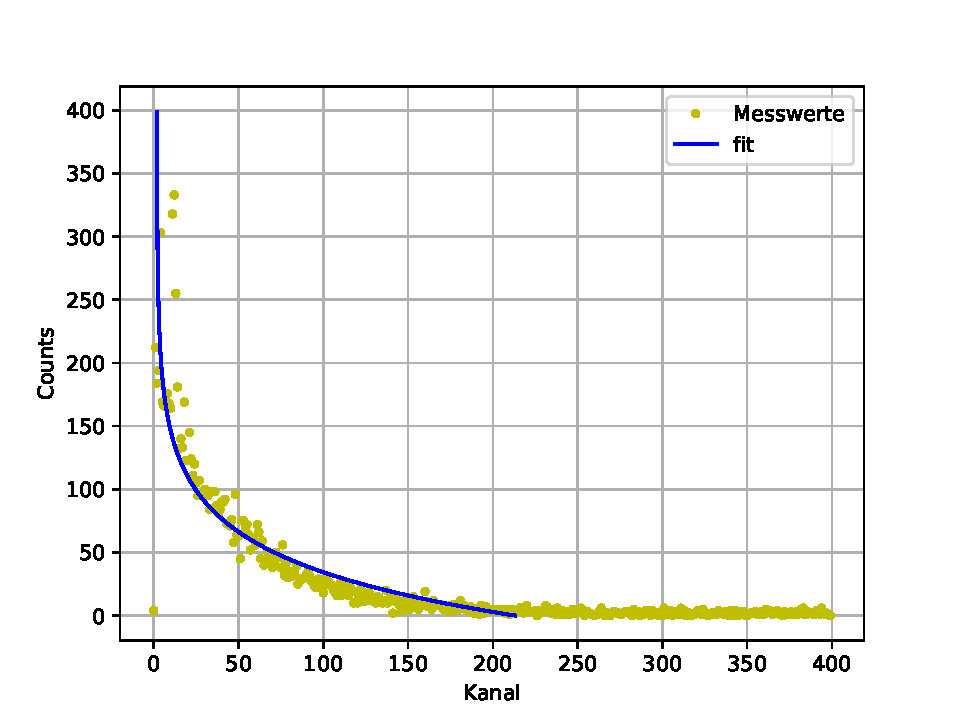
\includegraphics{./plots/lebensdauer.pdf}
  \caption{Gemessene Individuallebensdauern der detektierten Myonen}
  \label{fig:tau}
\end{figure}


Ein mittels $matplotlib$ \cite{matplotlib} über die Methode der kleinsten Quadrate durchgeführter ungewichteter Fit der Werte der Individuallebensdauern (dargestellt in Abb. \ref{fig:tau}) an eine Exponentialfunktion der Form $f(t) = A \exp\left(-\tau t\right)+U$ liefert folgende Werte:
\begin{align*}
  \tau &= \SI{2.03 \pm 0.09}{\micro\second} \\
  U &= 1.9 \pm 1.2 \\
  A &= 211 \pm 5
\end{align*}

Hierbei bezeichnet $U$ einen konstanten Untergrund aus zufällig, gleichverteilt auftretenden Ereignissen und $A$ als Ordinatenabschnitt.
Hierbei wurden die leeren ersten beiden Kanäle, sowie die ebenfalls leeren Kanäle 401 bis 511, bei der Auswertung der Daten vernachlässigt. Die ersten beiden Kanäle decken eine Zeit von ca. $t_{tot} = \SI{0.09}{\micro \second}$ ab.
Hierbei fällt auf, dass die Zahl der MCA gemessenen Ereignisse mit $C_{MCA}=10311.0$ geringer ist als die 10868 seperat gemessenen Stop Signale.


Mit $2096502$ detektierten Startimpulsen werden bei einer Messzeit von $\SI{96454}{\second}$ wird nach Gl. \eqref{eqn:barN} eine durchschnittliches Rauschen von $\SI{21.74}{\per \second}$ erwartet. Der Untergrund pro Kanal wird somit gemäß \eqref{eqn:Untergrund} mit $U = 1.7793 \pm 0.0025$ erwartet.


% \begin{figure}
%   \centering
%   \includegraphics{plot.pdf}
%   \caption{Plot.}
%   \label{fig:plot}
% \end{figure}



% \begin{table}
%    % Notation :  {% nicht entfernen ist sehr wichtig sonst Fehler !!
% \parbox{0.48\textwidth}{% %Ermöglicht zwei Tabellen neben einander
%   \centering
%   \sisetup{round-mode = places , round-precision = 0,scientific-notation=fixed, fixed-exponent = 0}
%          %rundet Werte aus Stelle, Stelle = ,  macht einen bestimmten festen exponenten
%   \resizebox{\textwidth}{!}{%  % skaliert zu große Tabellen
%   \begin{tabular}{S@{${}\pm{}$} S} % fügt plus minus Fehler Schreibweise hinzu
%     \toprule
%      $\text{e}_b / \si{\milli\meter}$ &
%      $\text{d}_b /\si{\milli\meter} $ & $\text{f}_b / \si{\milli\meter} $\\
%     \midrule
%     \bottomrule
%   \end{tabular}
%   % }
%   \caption{Tabellenunterschrift}
%   \label{tab:tab}
% }
% % \end{table}
% % \begin{table}
% \parbox{0.48\textwidth}{%
%   \centering
%   \sisetup{round-mode = places , round-precision = 0,scientific-notation=fixed, fixed-exponent = 0}
%   % \resizebox{\textwidth}{!}{%
%   \begin{tabular}{S@{${}\pm{}$} S}
%     \toprule
%      $\text{e}_b / \si{\milli\meter}$ &
%      $\text{d}_b /\si{\milli\meter} $ & $\text{f}_b / \si{\milli\meter} $\\
%     \midrule
%     \bottomrule
%   \end{tabular}
%   % }
%   \caption{Tabellenunterschrift}
%   \label{tab:tab}
% }
% \end{table}
